\chapter{Wykorzystane narzędzia, dokumentacja i kody pakietu $\mathcal{R}$ użyte w pracy}\label{docCoxSGD}
\section{Implementacje optymalizacji w regresji logistycznej}\label{kody}

\section{Model proporcjonalnych hazardów Coxa}\label{coxKody123}

\begin{Shaded}
\begin{Highlighting}[]
\NormalTok{checkArguments <-}\StringTok{ }\NormalTok{function(formula, data, learningRates,}
                             \NormalTok{beta_0, epsilon) \{}
  \KeywordTok{assert_that}\NormalTok{(}\KeywordTok{is.list}\NormalTok{(data) &}\StringTok{ }\KeywordTok{length}\NormalTok{(data) >}\StringTok{ }\DecValTok{0}\NormalTok{)}
  \KeywordTok{assert_that}\NormalTok{(}\KeywordTok{length}\NormalTok{(}\KeywordTok{unique}\NormalTok{(}\KeywordTok{unlist}\NormalTok{(}\KeywordTok{lapply}\NormalTok{(data, ncol)))) ==}\StringTok{ }\DecValTok{1}\NormalTok{)}
  \CommentTok{# + check names and types for every variables}
  \KeywordTok{assert_that}\NormalTok{(}\KeywordTok{is.function}\NormalTok{(learningRates))}
  \KeywordTok{assert_that}\NormalTok{(}\KeywordTok{is.numeric}\NormalTok{(epsilon))}
  \KeywordTok{assert_that}\NormalTok{(}\KeywordTok{is.numeric}\NormalTok{(beta_0))}
  
    \CommentTok{# check length of the start parameter}
  \NormalTok{if (}\KeywordTok{length}\NormalTok{(beta_0) ==}\StringTok{ }\DecValTok{1}\NormalTok{) \{}
    \NormalTok{beta_0 <-}\StringTok{ }\KeywordTok{rep}\NormalTok{(beta_0, }\KeywordTok{as.character}\NormalTok{(formula)[}\DecValTok{3}\NormalTok{] %>%}
\StringTok{                    }\KeywordTok{strsplit}\NormalTok{(}\StringTok{"}\CharTok{\textbackslash{}\textbackslash{}}\StringTok{+"}\NormalTok{) %>%}
\StringTok{                    }\NormalTok{unlist %>%}
\StringTok{                    }\NormalTok{length)}
  \NormalTok{\}}
  \KeywordTok{return}\NormalTok{(beta_0)}
\NormalTok{\}}
\end{Highlighting}
\end{Shaded}


\begin{Shaded}
\begin{Highlighting}[]
\NormalTok{prepareBatch <-}\StringTok{ }\NormalTok{function(formula, data) \{}
  \CommentTok{# Parameter identification as in  `survival::coxph()`.}
  \NormalTok{Call <-}\StringTok{ }\KeywordTok{match.call}\NormalTok{()}
  \NormalTok{indx <-}\StringTok{ }\KeywordTok{match}\NormalTok{(}\KeywordTok{c}\NormalTok{(}\StringTok{"formula"}\NormalTok{, }\StringTok{"data"}\NormalTok{),}
                \KeywordTok{names}\NormalTok{(Call), }\DataTypeTok{nomatch =} \DecValTok{0}\NormalTok{)}
  \NormalTok{if (indx[}\DecValTok{1}\NormalTok{] ==}\StringTok{ }\DecValTok{0}\NormalTok{) }
      \KeywordTok{stop}\NormalTok{(}\StringTok{"A formula argument is required"}\NormalTok{)}
  \NormalTok{temp <-}\StringTok{ }\NormalTok{Call[}\KeywordTok{c}\NormalTok{(}\DecValTok{1}\NormalTok{, indx)]}
  \NormalTok{temp[[}\DecValTok{1}\NormalTok{]] <-}\StringTok{ }\KeywordTok{as.name}\NormalTok{(}\StringTok{"model.frame"}\NormalTok{)}
  
  \NormalTok{mf <-}\StringTok{ }\KeywordTok{eval}\NormalTok{(temp, }\KeywordTok{parent.frame}\NormalTok{())}
  \NormalTok{Y <-}\StringTok{ }\KeywordTok{model.extract}\NormalTok{(mf, }\StringTok{"response"}\NormalTok{)}
  
  \NormalTok{if (!}\KeywordTok{inherits}\NormalTok{(Y, }\StringTok{"Surv"}\NormalTok{)) }
      \KeywordTok{stop}\NormalTok{(}\StringTok{"Response must be a survival object"}\NormalTok{)}
  \NormalTok{type <-}\StringTok{ }\KeywordTok{attr}\NormalTok{(Y, }\StringTok{"type"}\NormalTok{)}
  
  \NormalTok{if (type !=}\StringTok{ "right"} \NormalTok{&&}\StringTok{ }\NormalTok{type !=}\StringTok{ "counting"}\NormalTok{) }
      \KeywordTok{stop}\NormalTok{(}\KeywordTok{paste}\NormalTok{(}\StringTok{"Cox model doesn't support }\CharTok{\textbackslash{}"}\StringTok{"}\NormalTok{, type, }\StringTok{"}\CharTok{\textbackslash{}"}\StringTok{ survival data"}\NormalTok{, }
          \DataTypeTok{sep =} \StringTok{""}\NormalTok{))}
  
  \CommentTok{# collect times, status, variables and reorder samples }
  \CommentTok{# to make the algorithm more clear to read and track}
  \KeywordTok{cbind}\NormalTok{(}\DataTypeTok{event =} \KeywordTok{unclass}\NormalTok{(Y)[,}\DecValTok{2}\NormalTok{], }\CommentTok{# 1 indicates event, 0 indicates cens}
        \DataTypeTok{times =} \KeywordTok{unclass}\NormalTok{(Y)[,}\DecValTok{1}\NormalTok{],}
        \NormalTok{mf[, -}\DecValTok{1}\NormalTok{]) %>%}
\StringTok{    }\KeywordTok{arrange}\NormalTok{(times) }
\NormalTok{\}}
\end{Highlighting}
\end{Shaded}

%dokumentacja funkcji coxphSGD
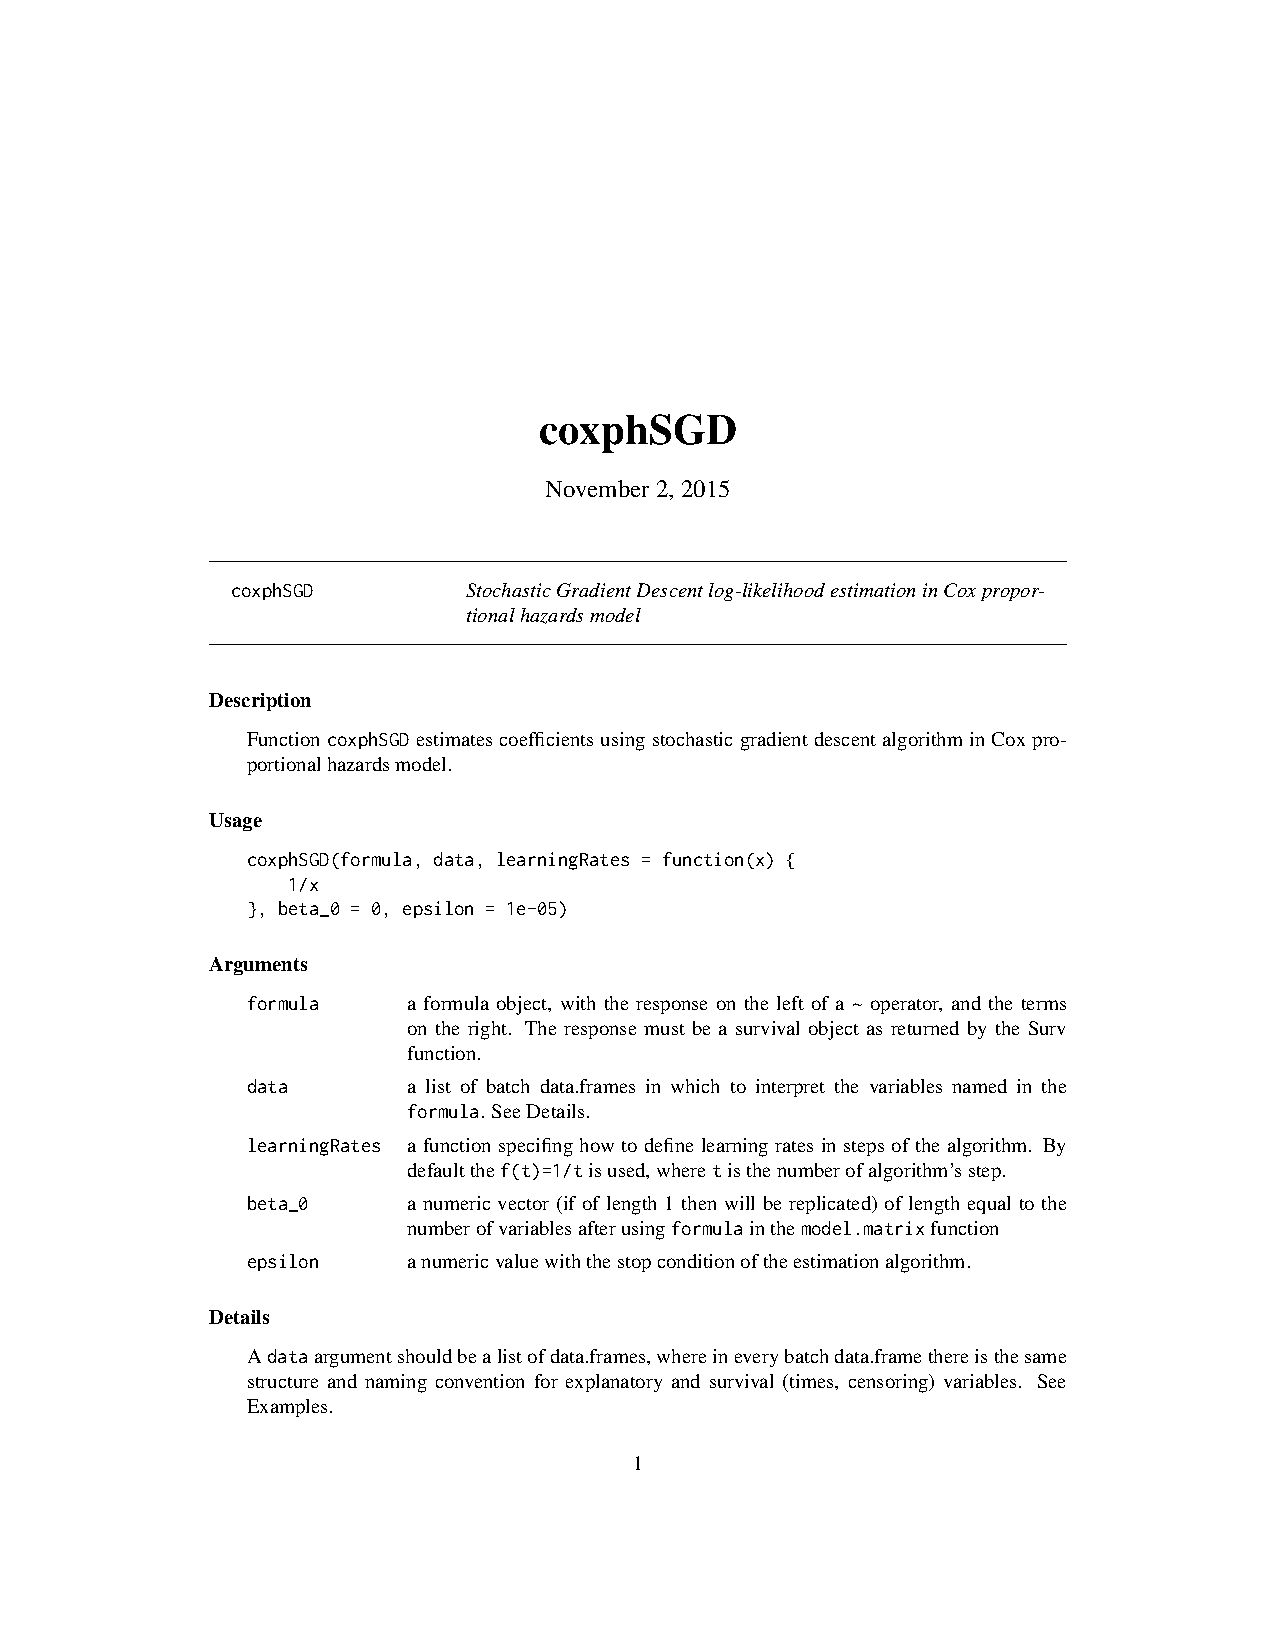
\includepdf[pages=-]{coxphSGD3.pdf}
%\chapter{Dokumentacja pakietu RTCGA}
%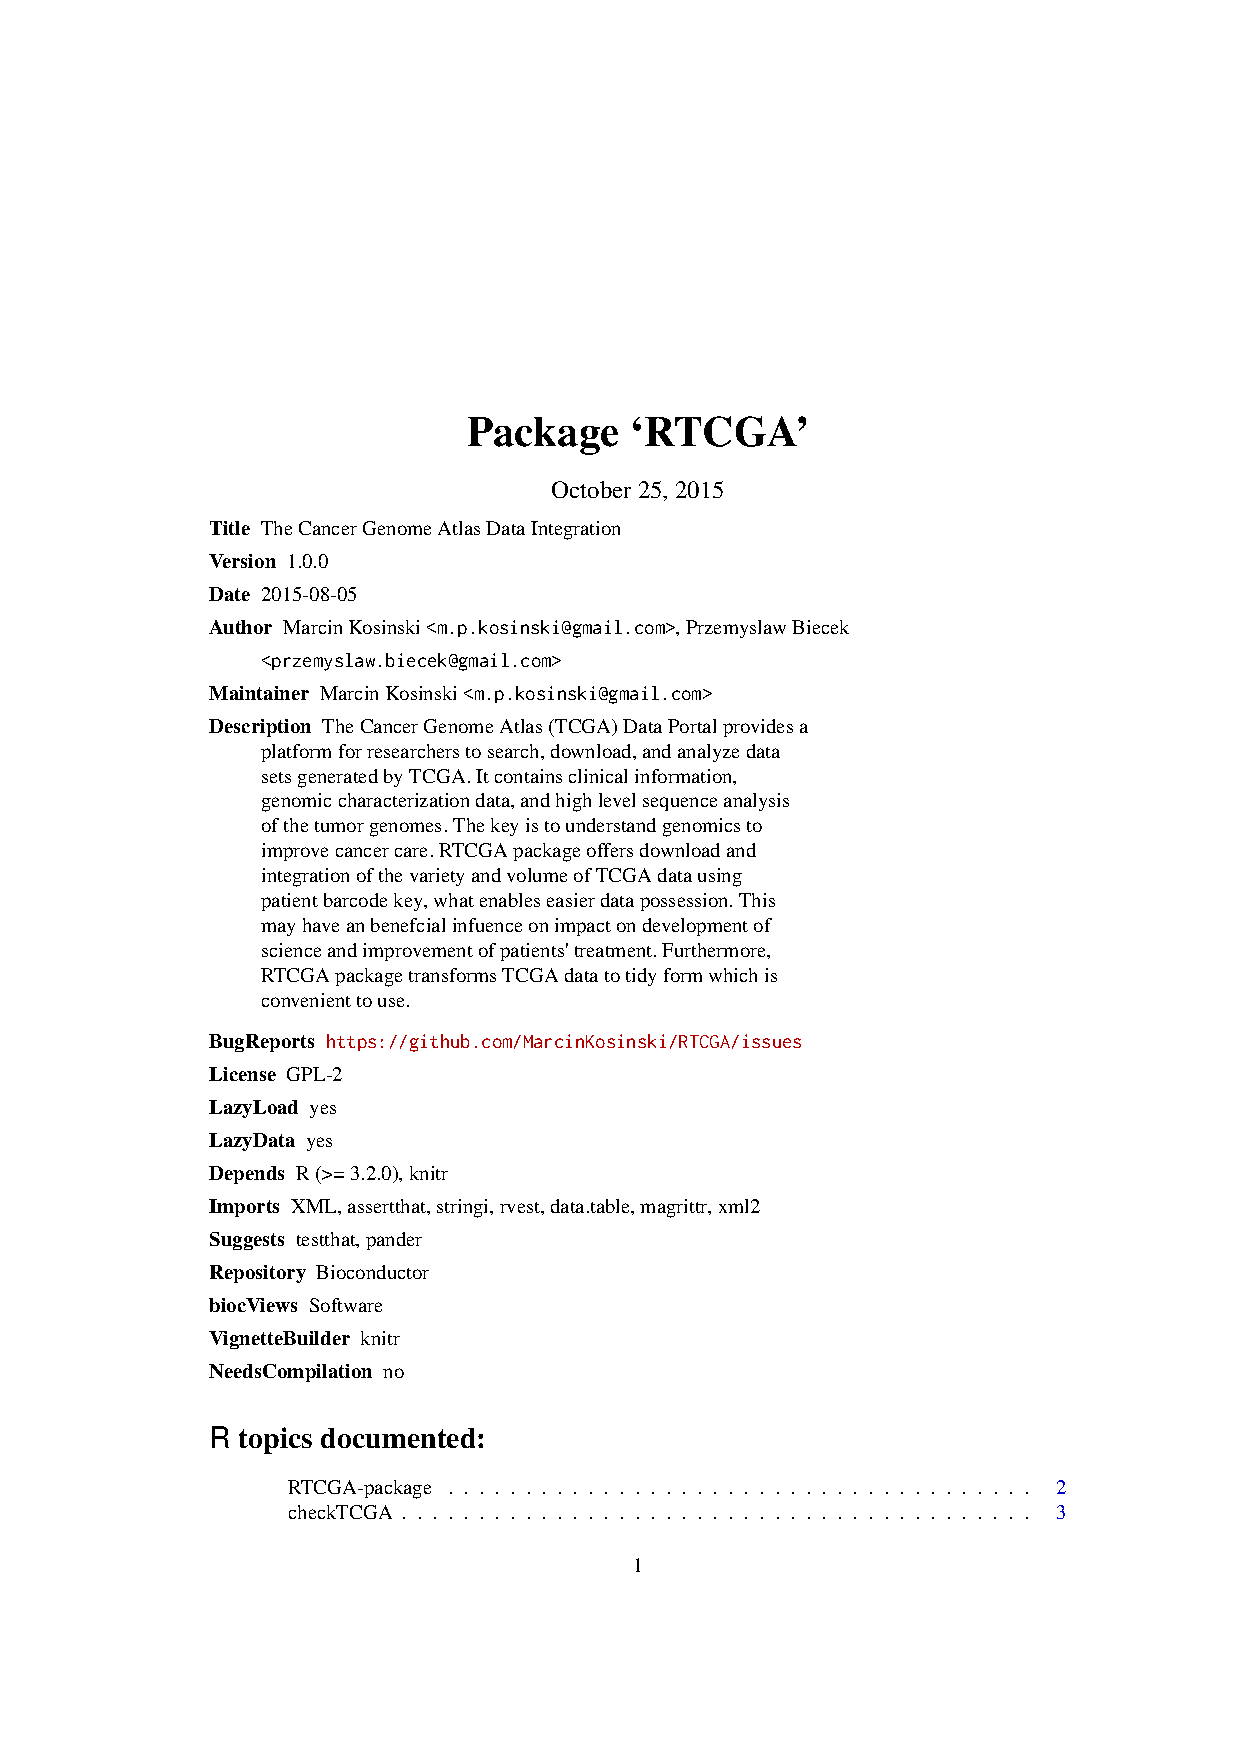
\includepdf[pages=-]{RTCGA.pdf}